\begin{enumerate}[label=\thechapter.\arabic*,ref=\thechapter.\theenumi]
\numberwithin{equation}{enumi}
\numberwithin{figure}{enumi}
\numberwithin{table}{enumi}
\item 
	Construct a triangle $ABC$ in which $a, \angle{B}$ and $c + b  = K$ are given.
\label{cons/tri/1}
	\\
	\solution 
\iffalse
\documentclass[10pt,a4paper]{report}
\usepackage[latin1]{inputenc}
\usepackage{amsmath}
\usepackage{amsfonts}
\usepackage{amssymb}
\usepackage{graphicx}
\usepackage{hyperref}
\usepackage{multicol}
\usepackage[margin=0.1 in]{geometry}
\usepackage{tikz}
\usepackage{romannum}
\usepackage{listings}
\usetikzlibrary{arrows,shapes.gates.logic.US,shapes.gates.logic.IEC,calc}
\usepackage{titlesec}
\titlespacing{\subsection}{1pt}{\parskip}{3pt}
\titlespacing{\subsubsection}{0pt}{\parskip}{-\parskip}
\titlespacing{\paragraph}{0pt}{\parskip}{\parskip}
\newcommand{\myvec}[1]{\ensuremath{\begin{pmatrix}#1\end{pmatrix}}}
\let\vec\mathbf

\begin{document}

\centering {
\includegraphics[scale=0.07]{IITH.png}} \vspace{3mm}\\ \raggedleft Name:T.Manasa Reddy\vspace{2mm}\\ \raggedleft Roll No.: FWC22048\vspace{2mm}\\ \raggedright Sep 2022 \hspace{12cm} \raggedleft manasatanuboddi@gmail.com \vspace{10mm}
\\ \centering \Large \textbf{MATRIX ASSIGNMENT} \normalsize \vspace{15mm}

\begin{multicols}{2}
\section{Problem:}  
\fi
	\iffalse
	See Fig. 
		\ref{eq:cons/tri/9/11/2/1}.
	\begin{figure}[!h]
		\centering
 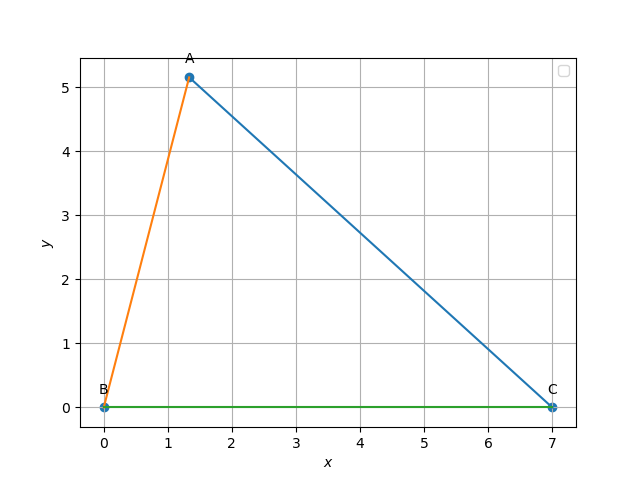
\includegraphics[width=\columnwidth]{chapters/9/11/2/1/figs/Figure_1.png}
		\caption{}
		\label{eq:cons/tri/9/11/2/1}
  	\end{figure}
	
	\vspace{3mm}
\section{Solution}
The input parameters for this construction are
\begin{center}
\begin{tabular}{|c|c|c|}
	\hline
	\textbf{Symbol}&\textbf{Value}&\textbf{Description}\\
	\hline
	BC & a & where a is 7cm\\
	\hline
	AB & b & AB distance is b \\
	\hline 
	AC & c & AC distance is c \\
	\hline
	$\angle{BC}$ & $75^0$ &  $\triangle$ABC \\
	\hline
	$\vec{C}$ & $\myvec{a\\0}$ & BC length is equal to a\\
	\hline
	$\vec{A}$ & $\myvec{ \cos\theta \\ \sin\theta}$ & using the cosine formula in $\triangle$ABC\\
	\hline
\end{tabular}
\end{center}
\raggedright {termux commands :}
\begin{center}
\fbox{\parbox{8.5cm}{bash line.sh.........using shell command}}
\end{center}
\raggedright\textbf{Caluclating Other Coordinate: } \\
\raggedright Let the coordinates of A are $X_{2}$,$Y_{2}$ respectively. \\
  \raggedright Let \textbf{A} =
  $\begin{pmatrix} 
 \cos \theta\\
  \sin\theta \\
\end{pmatrix}$ \\
\raggedright 
\fi
	Using the cosine formula in  $\triangle ABC$,
\begin{align}
	{b}^2&= {a}^2 + {c}^2 - 2ac\cos{B}
\\
\implies	(b+c)(b-c) &= {a}^2- 2  a  c\cos{B}
\\
	\text{or, }K(b-c) &= {a}^2- 2  a  c\cos{B}
		\label{eq:cons/tri/9/11/2/1/k}
\end{align}
%
where
\begin{align}
K = b+c 
		\label{eq:cons/tri/9/11/2/1/k/def}
\end{align}
From 
		\eqref{eq:cons/tri/9/11/2/1/k}
		and
		\eqref{eq:cons/tri/9/11/2/1/k/def},
\begin{align}
	\myvec{
		1 & 1
		\\
		1 & -1 
	}
	\myvec{
	b
	\\
	c
	}
	&=
	\myvec{
		\frac{{a}^2- 2  a  c\cos{B}}{K}
		\\
K}
\\
\implies
	\myvec{
	b
	\\
	c
	}
	&=
	\frac{1}{2}\myvec{
		1 & 1
		\\
		1 & -1 
	}
	\myvec{
		\frac{{a}^2- 2  a  c\cos{B}}{K}
	\\
K}
		\label{eq:cons/tri/9/11/2/1/k/mateq}
\\
\because
\myvec{
		1 & 1
		\\
		1 & -1 }
	\myvec{
		1 & 1
		\\
		1 & -1 }
	&	= 	{2}\vec{I}
\end{align}
From 
		\eqref{eq:cons/tri/9/11/2/1/k/mateq}
\begin{align}
	c
	&=
	\frac{1}{2}\vec{e}_2^{\top}\myvec{
		1 & 1
		\\
		1 & -1 
	}
	\myvec{
		\frac{{a}^2}{K}
	\\
	K}- \frac{2  a  c\cos{B}}{K}
\\
\implies
	c &=
	\frac{1}{2\brak{1+ \frac{2  a  \cos{B}}{K}}}\vec{e}_2^{\top}\myvec{
		1 & 1
		\\
		1 & -1 
	}
	\myvec{
		\frac{{a}^2}{K}
	\\
K}
\end{align}
The coordinates of $\triangle ABC$ can then be expressed as
\begin{align}
	\vec{A}=c\myvec{\cos B \\ \sin B},
	\vec{B} = \vec{0},
	\vec{C} =\myvec{a \\ 0}.
\end{align}
\iffalse
   reduced row echelon form of $\begin{pmatrix}13 & -13 + \frac{\sqrt{2} (-7 + 7 \sqrt{3})}{2} & 49\\1 & 1 & 13\end{pmatrix}$
        \vspace{3mm}
        \\Divide row1 by 13: R1 = $\frac{R1}{13}$
        \vspace{7mm}
 $        \begin{pmatrix} 1 & -\frac{ -7\sqrt{6}  + 7 \sqrt{2} + 26 )}{26} & \frac{49}{13}\\ 1& 1 & 13\end{pmatrix}$ \vspace{5mm}
        \\ Subtract row 1 from row 2: R2 = R2 - R1 \vspace{3mm}
        \\ $\begin{pmatrix}1 & -\frac{ -7\sqrt{6}  + 7 \sqrt{2} + 26 )}{26} & \frac{49}{13}\\ 0 & -\frac{ -7\sqrt{6}  + 7 \sqrt{2} + 52 )}{26} & \frac{120}{13}\end{pmatrix}$ \vspace{6mm}
         Multiply row 2 by $\frac{26}{- 7 \sqrt{6} + 7 \sqrt{2} + 52}$:\vspace{3mm}
         R2=$\frac{26}{- 7 \sqrt{6} + 7 \sqrt{2} + 52}$  
         \vspace{6mm}
    \\ Add row 2 multiplied by $\frac{- 7 \sqrt{6} + 7 \sqrt{2} + 26}{26}$ \vspace{5mm}
     \\  $\begin{pmatrix}1 & 0 &-\frac{ 91\sqrt{6}  + 91\sqrt{2} + 436)}{-7\sqrt{6}  + 7 \sqrt{2} + 52 )}\\ 0 & 1 &\frac{240}{ -7\sqrt{6} + 7 \sqrt{2} + 52} \end{pmatrix} $ \vspace{5mm}
     \\ $\begin{pmatrix}
     b \\
     c \\
     \end{pmatrix}$%
     = $\begin{pmatrix}
     -\frac{ 91\sqrt{6}  + 91\sqrt{2} + 436)}{-7\sqrt{6}  + 7 \sqrt{2} + 52 )} \\
     \frac{240}{ -7\sqrt{6} + 7 \sqrt{2} + 52}
     \end{pmatrix}$%
     \vspace{5mm}
    \\ \raggedright \textbf{A} = c$\begin{pmatrix}
                 \cos 75 \\ 
                 \sin 75 \\
              \end{pmatrix}$%
              =$\begin{pmatrix}
                 1.33 \\
                 5.15 \\
                 \end{pmatrix}$%
                 \vspace{5mm}
              \\ \raggedright  \textbf{B} = $\begin{pmatrix}
                 0\\
                 0\\
              \end{pmatrix}$% 
              \vspace{5mm}
             \\ \raggedright  \textbf{C} = $\begin{pmatrix}
                  7\\
                  0\\
              \end{pmatrix}$%
              \vspace{5mm}
\\
Below python code realizes the above construction : 
\fbox{\parbox{8.5cm}{\url{https://github.com/manasareddy442002/fwc-moudle1/blob/matrix-lines/matrix.py}}}

 \section{Construction}
 	\begin{center}
  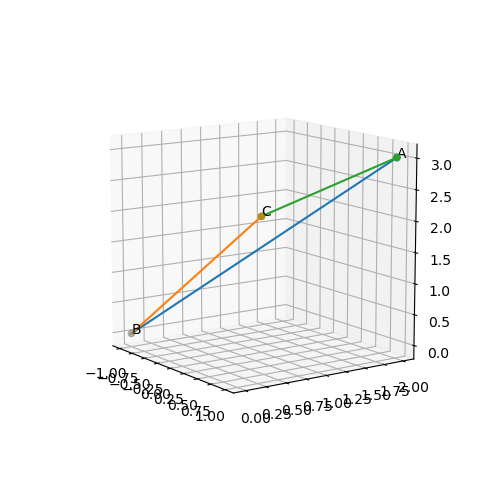
\includegraphics[scale=0.5]{Figure_1.png}
  	\end{center}
\vspace{3cm}
\end{multicols}

\end{document}
\fi

%
\iffalse
\item 
\label{cons/tri/2}
\iffalse
\documentclass[10pt,a4paper]{report}
\usepackage[latin1]{inputenc}
\usepackage{amsmath}
\usepackage{amsfonts}
\usepackage{amssymb}
\usepackage{graphicx}
\usepackage{hyperref}
\usepackage{multicol}
\usepackage[margin=0.5in]{geometry}
\usepackage{tikz}
\usepackage{romannum}
\usepackage{listings}
\usetikzlibrary{arrows,shapes.gates.logic.US,shapes.gates.logic.IEC,calc}
\usepackage{titlesec}
\titlespacing{\subsection}{1pt}{\parskip}{3pt}
\titlespacing{\subsubsection}{0pt}{\parskip}{-\parskip}
\titlespacing{\paragraph}{0pt}{\parskip}{\parskip}
\newcommand{\myvec}[1]{\ensuremath{\begin{pmatrix}#1\end{pmatrix}}}
\let\vec\mathbf

\begin{document}

\centering {
\includegraphics[scale=0.07]{IIT.png}} \vspace{3mm}\\ \raggedleft Name:Somisetty.Kedareswari\vspace{2mm}\\ \raggedleft Roll No.: FWC22049\vspace{2mm}\\ \raggedright Sep 2022 \hspace{12cm} \raggedleft mail2kedari@gmail.com \vspace{10mm}
\\ \centering \Large \textbf{MATRIX ASSIGNMENT} \normalsize \vspace{15mm}
\begin{multicols}{2}
\section{Problem:}  
\fi
	Construct a triangle $ABC$ in which $BC=8cm, \angle{B}=45\degree$ and $AB - AC = 3.5 cm$.
	\solution 
	See Fig. 
		\ref{fig:9/11/2/2}.
	\begin{figure}[!h]
		\centering
 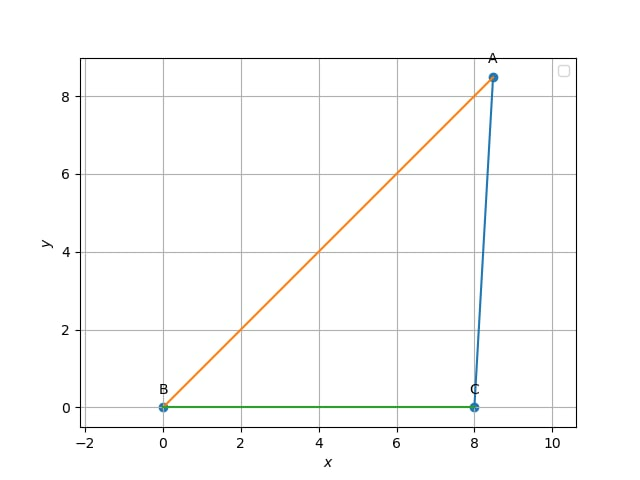
\includegraphics[width=\columnwidth]{chapters/9/11/2/2/figs/Fig.png}
		\caption{}
		\label{fig:9/11/2/2}
  	\end{figure}
	Using the cosine formula in  $\triangle ABC$,
\begin{align}
	{b}^2&= {a}^2 + {c}^2 - 2ac\cos{B}
\\
\implies	(b+c)(b-c) &= {a}^2- 2  a  c\cos{B}
\\
	\text{or, }K(b+c) &= {a}^2- 2  a  c\cos{B}
		\label{fig:9/11/2/2/k}
\end{align}
%
where
\begin{align}
-K = b-c 
		\label{fig:9/11/2/2/k/def}
\end{align}
From 
		\eqref{fig:9/11/2/2/k}
		and
		\eqref{fig:9/11/2/2/k/def},
\begin{align}
	\myvec{
		1 & 1
		\\
		1 & -1 
	}
	\myvec{
	b
	\\
	c
	}
	&=
	\myvec{
		\frac{{a}^2- 2  a  c\cos{B}}{K}
		\\
-K}
\\
\implies
	\myvec{
	b
	\\
	c
	}
	&=
	\frac{1}{2}\myvec{
		1 & 1
		\\
		1 & -1 
	}
	\myvec{
		\frac{{a}^2- 2  a  c\cos{B}}{K}
	\\
-K}
		\label{fig:9/11/2/2/k/mateq}
\\
\because
\myvec{
		1 & 1
		\\
		1 & -1 }
	\myvec{
		1 & 1
		\\
		1 & -1 }
	&	= 	{2}\vec{I}
\end{align}
From 
		\eqref{fig:9/11/2/2/k/mateq}
\begin{align}
	c
	&=
	\frac{1}{2}\vec{e}_2^{\top}\myvec{
		1 & 1
		\\
		1 & -1 
	}
	\myvec{
		\frac{{a}^2}{K}
	\\
	-K}- \frac{2  a  c\cos{B}}{K}
\\
\implies
	c &=
	\frac{1}{2\brak{1+ \frac{2  a  \cos{B}}{K}}}\vec{e}_2^{\top}\myvec{
		1 & 1
		\\
		1 & -1 
	}
	\myvec{
		\frac{{a}^2}{K}
	\\
-K}
\end{align}
The coordinates of $\triangle ABC$ can then be expressed as
\begin{align}
	\vec{A}=c\myvec{\cos B \\ \sin B},
	\vec{B} = \vec{0},
	\vec{C} =\myvec{a \\ 0}.
\end{align}

	\iffalse
\section{Solution}
The input parameters for this construction are
\begin{center}
\begin{tabular}{|c|c|c|}
  \hline
  \textbf{Symbol}&\textbf{Value}&\textbf{Description}\\
  \hline
  BC & a & where a is 8cm\\
  \hline
  $\angle{BC}$ & $45^0$ &  $\Delta$ABC \\
  \hline
  k & 3.5 & constant value\\
  \hline
\end{tabular}
\end{center}
\raggedright\textbf{Caluclating Other Coordinate: } \\
\raggedright The coordinates of B and C are $X_{2}$,$Y_{2}$ respectively. \\
  \raggedright Let \textbf{A} = c$\times$
  $\begin{pmatrix} 
 \cos \theta\\
  \sin\theta \\
\end{pmatrix}$ \\
\raggedright Using the Cosine formula in  $\Delta$ABC, \\ \vspace{3mm}
\begin{equation}
{b}^2\hspace{1.5cm}= {a}^2 + {c}^2 - 2accos\vec{B}
\end{equation}
\begin{equation}
(b+c)(b-c) = {a}^2- 2accos\vec{B}
\end{equation}
Given
\begin{equation}
        c-b=k
\end{equation}\\
Upon Simplifaction we get:- \\
\begin{equation}
  (b+c)(-k) = {a}^2- 2accos\vec{B} 
\end{equation}
\begin{equation}
-kc-kb+2accos\vec{B}= {a}^2
\end{equation}
\begin{equation}
-kb-c(-k+2acos\vec{B})= {a}^2
\end{equation}
     From the above, we obtain the matrix equation:- \\ \vspace{3mm}
        $\begin{pmatrix}
            -k & k+2acos\vec{B}  \\
            -1 & 1  \\
        \end{pmatrix}$% 
        $\begin{pmatrix}
            c \\
            b \\
        \end{pmatrix}$% 
           =
           $\begin{pmatrix}
            k\\
            a^2\\
        \end{pmatrix}$%   
        \vspace{5mm}           
   \\  
    $\begin{pmatrix}
            -3.5 & 3.5+2(8)cos45^0 \\
            -1 & 1  \\
        \end{pmatrix}$% 
        $\begin{pmatrix}
            c \\
            b \\
        \end{pmatrix}$% 
           =
           $\begin{pmatrix}
            3.5\\
            64\\
        \end{pmatrix}$%   
        \vspace{5mm}           
   \\  
   Augmented Matrix $\implies$
   $\begin{pmatrix}
         -3.5 & 3.5+2(8)cos45^0 & 3.5\\
            -1 & 1  & 64\\
          \\
    \end{pmatrix}$%
    \\
    Reducing to echelon form:-
   \\
    $\begin{pmatrix}
    \myvec{1&-1&\frac{7}{2} \\ -\frac{7}{2}&\frac{78154172560113}{10000000000000}&64}
    \xleftarrow[]{-R_1 \leftarrow R_1}
    \end{pmatrix}$%
  \\
  \vspace{5mm}
   $\begin{pmatrix}
    \myvec{1&-1&\frac{7}{2} \\ 0&1&\frac{517500000000000}{43154172560113}}
    \xleftarrow[]{\frac{10000000000000R2}{43154172560113} \leftarrow R_2}
    \end{pmatrix}$%
  \\
  \vspace{5mm}
  $\begin{pmatrix}
    \myvec{1&0&\frac{732920792079209}{86308345120226} \\ 0&1&\frac{517500000000000}{43154172560113}}
    \xleftarrow[]{R1+R2 \leftarrow R_2}
    \end{pmatrix}$%
  \\
  \vspace{5mm}
  Reduced Echelon Form: 
  $\begin{pmatrix}
    \myvec{1&0&8.491887905604763 \\ 0&1&11.991887905604763}
    \end{pmatrix}$% 
    \\
    \vspace{5mm}
      $\begin{pmatrix}
            c\\
            b\\
        \end{pmatrix}$% 
            =
            $\begin{pmatrix}
            11.99\\
            8.49\\
        \end{pmatrix}$% 
        \vspace{3mm}
   \\  The vertices of $\Delta$ ABC are \\ \vspace{3mm}
     \raggedright \textbf{A} = 11.99$\begin{pmatrix}
                 cos 45 \\ 
                 sin 45 \\
              \end{pmatrix}$%
              =$\begin{pmatrix}
                 8.4 \\
                 8.4 \\
                 \end{pmatrix}$%
                 \vspace{5mm}
              \\ \raggedright  \textbf{B} = $\begin{pmatrix}
                 0\\
                 0\\
              \end{pmatrix}$% 
              \vspace{5mm}
             \\ \raggedright  \textbf{C} = $\begin{pmatrix}
                  8\\
                  0\\
              \end{pmatrix}$%
              \\
Below python code realizes the above construction : 
\fbox{\parbox{8.5cm}{\url{https://github.com/kedareswari200/fwc-moudle1/blob/Matri_lines/triangle.py}}}
 \\
 \section{Construction}
   \begin{center}
  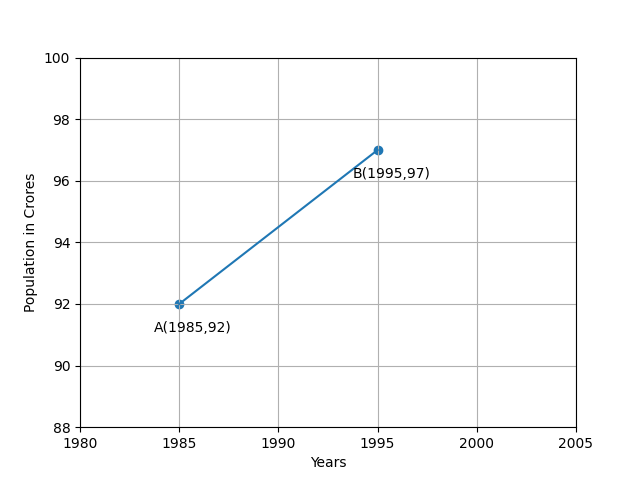
\includegraphics[scale=0.5]{Fig.png}
    \end{center}
\vspace{3cm}
\end{multicols}

\end{document}
\fi

%
\item 
\label{cons/tri/3}
\iffalse
\documentclass[10pt,a4paper]{article}
\usepackage{amsmath}
\usepackage{amsfonts}
\usepackage{amssymb}
\usepackage{graphicx}
\usepackage{multicol}
\usepackage{tabularx}
\usepackage{tikz}
\usetikzlibrary{arrows,shapes,automata,petri,positioning,calc}
\usepackage{hyperref}
\usepackage{tikz}
\usepackage{gensymb}
\usepackage{polynom}
\usetikzlibrary{matrix,calc}
\makeatletter
\newcommand\xleftrightarrow[2][]{%
  \ext@arrow 9999{\longleftrightarrowfill@}{#1}{#2}}
\newcommand\longleftrightarrowfill@{%
  \arrowfill@\leftarrow\relbar\rightarrow}
\makeatother
\usepackage[margin=0.5in]{geometry}
\newcommand{\myvec}[1]{\ensuremath{\begin{pmatrix}#1\end{pmatrix}}}
\let\vec\mathbf
\newenvironment{Figure}
  {\par\medskip\noindent\minipage{\linewidth}}
  {\endminipage\par\medskip}
\begin{document}
%--------------------logo figure-------------------------%
\begin{figure*}[!tbp]
 \centering
  \begin{minipage}[b]{0.4\textwidth}
  
\includegraphics[scale=.25]{iitlogo.png} 
  \end{minipage}
\end{figure*}
%--------------------name & rollno-----------------------
\raggedright \textbf{Name}:\hspace{1mm} Ganga Gopinath\hspace{3cm} \Large \textbf{Matrix Assignment}\hspace{2.5cm} % 
\normalsize \textbf{Roll No.} :\hspace{1mm} FWC22050\vspace{1cm}
\begin{multicols}{2}
\section{Problem statement:}
\fi
	Construct a triangle $PQR$ in which $QR=6cm, \angle{Q}=60\degree$ and $PR - PQ = 2cm$.
	\begin{figure}[!h]
		\centering
 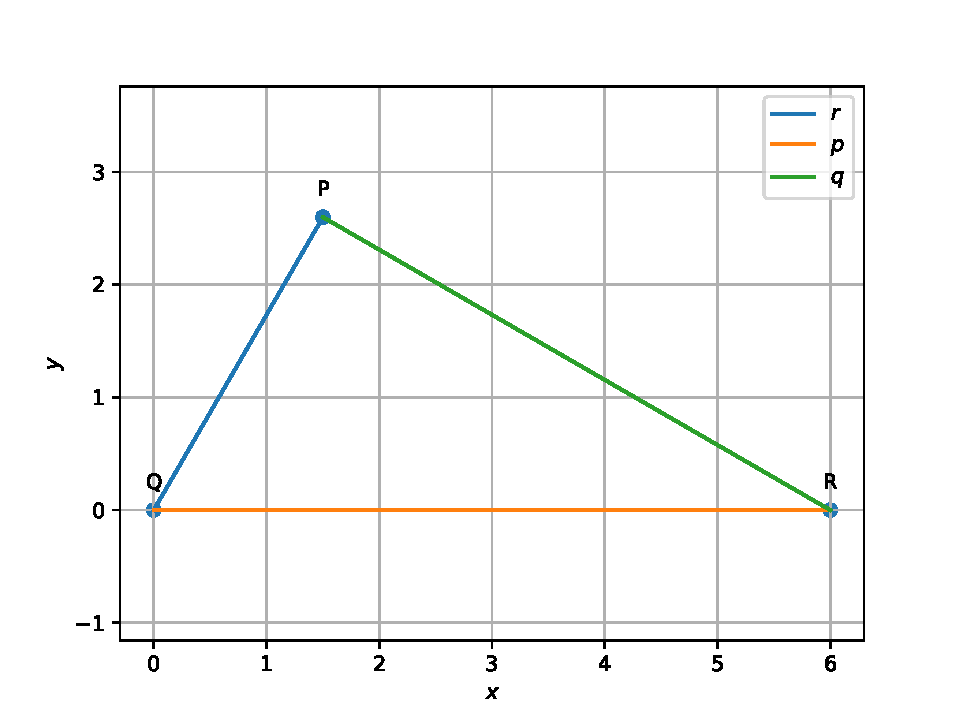
\includegraphics[width=\columnwidth]{chapters/9/11/2/3/figs/line1.pdf}
		\caption{}
		\label{fig:9/11/2/3}
  	\end{figure}
	\solution  Same as Problem 
\ref{chapters/9/11/2/1} with 
\begin{align}
\angle Q = \angle B, QR = a, PR = b, PQ = c
\end{align}
\iffalse

\textbf{Law of Cosines}
\vspace{2mm}\raggedright \\

The law of Cosines relates the length of the triangle to the cosines of one of its angles. It states that, if the length of two sides and the angle between them is known for a triangle, then we can determine the length of the third side. It is given by:
\begin{equation}
\alpha^2=\beta^2+\gamma^2-2\beta\gamma\cos\theta
\end{equation}
%-----------------------------solution---------------------------
\raggedright \textbf{SOLUTION}:\vspace{5mm}\\
\raggedright \textbf{Steps of Construction:}\vspace{2mm}\\
\textbf{Step 1:}\vspace{2mm}\\
Let P,Q and R be the vertices of the triangle  with coordinates.

Given QR length is a=6cm,
So the coordinates of vertices  Q,R and P are :\vspace{2mm}\\
\begin{center}$
{
 Q =\begin{pmatrix}
0 \\
0 
\end{pmatrix} 
\vspace{1mm}
R=\begin{pmatrix}
6 \\
0 
\end{pmatrix} 
\vspace{1mm}
P=\alpha\begin{pmatrix}
cos \theta\\
  sin \theta\\
\end{pmatrix} }
\vspace{1mm}$
\end{center}
Also given the angle is $Q=60^0$,so by finding the coordinates of the other sid
    e we can form a required triangle. \\
 \vspace{2mm}
For the input parameters in Table 1.\\
{\setlength\extrarowheight{2pt}
\begin{center}
\begin{tabular}{|c|c|c|}
	\hline
	\textbf{Symbol}&\textbf{Value}&\textbf{Description}\\
	\hline
	Q&$\begin{pmatrix}
	0\\0\\
	\end{pmatrix} $& Q Point\\
	\hline
	R&$\begin{pmatrix}
	6\\0\\
	\end{pmatrix} $& R Point\\
	\hline
	$\theta$&60$^{\circ}$&$\angle$PQR\\
	\hline
	$\lambda$ & 2 & PR-PQ\\
	\hline
	q&$\alpha$  & PR\\
	\hline
	r &$\gamma$  & PQ\\
	\hline
	p & 6 & QR\\
	\hline
\end{tabular}
%}\\
\\ {Table 1}\\
\end{center}
\vspace{3mm} 
Given that,
\begin{equation}
	\alpha-\gamma=2
\end{equation}
By using the Cosine formula in  $\Delta$PQR \\ 
\begin{equation}
\alpha^2=\beta^2+\gamma^2-2\beta\gamma\cos\theta 
\end{equation}
\vspace{1mm}
\begin{equation}
\alpha^2-\gamma^2=\beta^2-2\beta\gamma\cos\theta
\end{equation}
\vspace{1mm}
\begin{equation}
(\alpha+\gamma)(\alpha-\gamma)=\beta^2-2\beta\gamma\cos\theta
\end{equation}
\vspace{1mm}
\begin{equation}
(\alpha+\gamma)(\lambda)=\beta^2-2\beta\gamma\cos\theta
\end{equation}
\vspace{1mm}
\begin{equation}
\lambda\alpha +\lambda \gamma +2\beta\gamma\cos\theta=\beta^2
\end{equation}
\vspace{1mm}
\begin{equation}
\lambda \alpha +\gamma(\lambda+2\beta\cos\theta)=\beta^2
\end{equation}
\vspace{1mm}
%\begin{center}
%	$0=6^2+\gamma^2 -\alpha^2-2\times \gamma \times 6 \times cos60$\\

%\vspace{5mm}
%\end{center}
%After simplification
%\begin{equation}
%	   4\gamma+\alpha =18
%\end{equation}

\textbf{Step 2:}\vspace{2mm}\\
We know that,\\
\begin{equation}
\vec{A  X = B}
\end{equation}
Using equation (2) and (8),


\begin{equation}
  \begin{pmatrix}
1 & -1\\
\lambda & \lambda+2\beta\cos\theta
\end{pmatrix} 
\begin{pmatrix}
\alpha\\
\gamma
\end{pmatrix} 
=
\begin{pmatrix}
\lambda\\ 
 \beta^2\
\end{pmatrix}
\end{equation}\vspace{2mm}\\
 
After substituting values,
\begin{equation}
  \begin{pmatrix}
1 & -1\\
1 &4
\end{pmatrix} 
\begin{pmatrix}
\alpha\\
\gamma
\end{pmatrix} 
=
\begin{pmatrix}
2\\ 
 18\
\end{pmatrix}
\end{equation}\vspace{2mm}\\


The augmented matrix for the above matrix equation is 
\vspace{3mm}
\begin{equation}
\begin{pmatrix}
  1 & -1 & \vrule & 2\\
  1 & 4  &\vrule & 18
    \end{pmatrix}  
    \end{equation} 
    
  \begin{center}
  $ \xleftrightarrow{\text{$R_2$ $\leftarrow {R_2}-{R_1}$}} $
$\begin{pmatrix}
 1 & -1& \vrule & 2\\
 0 & 5  &\vrule & 16\
  \end{pmatrix}$
  \\
  \end{center}
  
  \begin{center}
$ \xleftrightarrow{\text{$R_2$ $\leftarrow  \frac{1}{5}{R_2}$}} $
$\begin{pmatrix}
 1 & -1 & \vrule & 2\\
  0 & 1  &\vrule & \frac{16}{5}\
  \end{pmatrix}$
  \\
  \end{center}    
  
  \begin{center}
  $ \xleftrightarrow{\text{$R_1$ $\leftarrow  {R_1}+{R_2}$}} $
$\begin{pmatrix}
  1 & 0 & \vrule & \frac{26}{5}\\
  0 & 1  &\vrule & \frac{16}{5}\
  \end{pmatrix}$
  \\
  \end{center}

  \begin{equation}
\implies X = 
   \begin{pmatrix}
   \frac {26}{5}\\ 
   \frac{16}{5}
 \end{pmatrix}
 \end{equation}
Using equation (7) we get ,
\begin{equation}
	\alpha = \frac{26}{5} \vspace{2mm}
\end{equation}
\begin{equation}
	\gamma= \frac{16}{5}\vspace{2mm}
\end{equation}
The vertices of $\Delta$ PQR are \\
\begin{equation}
P= \frac{26}{5} \begin{pmatrix}
cos 60\\
sin 60\\
\end{pmatrix} 
,Q= \begin{pmatrix}
 0\\
 0\\
 \end{pmatrix} 
,R= \begin{pmatrix}
 6\\
 0\\
\end{pmatrix} 
\end{equation} \vspace{2mm}


\textbf{Result} 
\begin{center}
	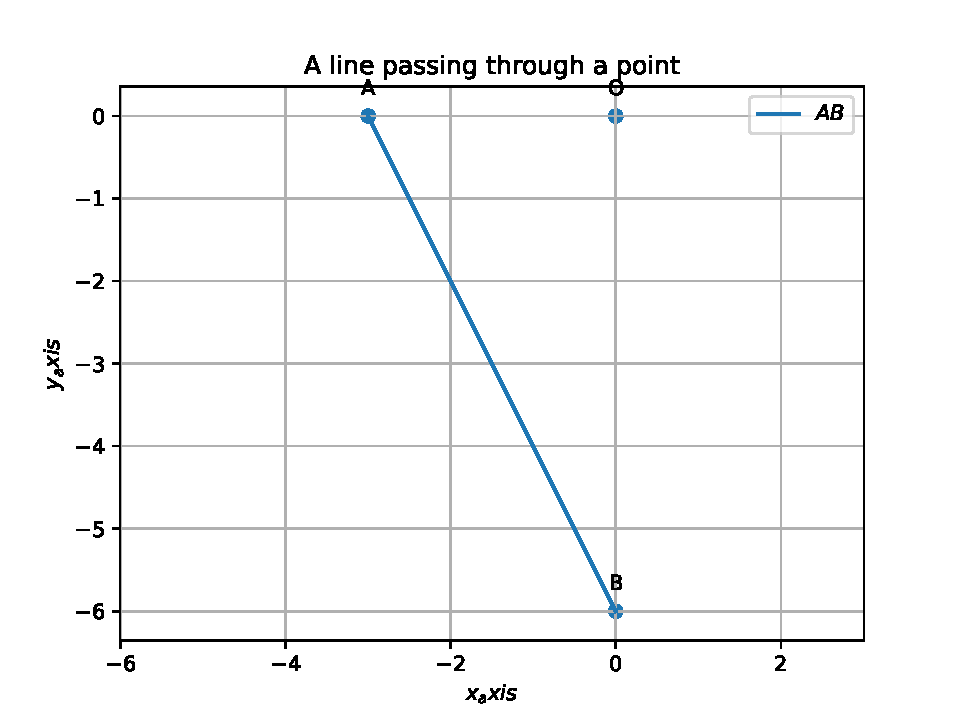
\includegraphics[width=0.4\textwidth]{line1.pdf}
\end{center}\vspace{5mm}

\vspace{4mm}  
\textbf{Implementation}
\begin{center}
\setlength{\arrayrulewidth}{0.5mm}
\setlength{\tabcolsep}{5pt}
\renewcommand{\arraystretch}{3}
    \begin{tabular}{|l|c|}
    \hline 
    \textbf{Equation no} & \textbf{Role} \\ \hline
    1 &  law of Cosines \\ 
    7 & Matrix form of Linear equation  \\
    10 & Length of r\\
    11& Length of q \\
    
    \hline
      \end{tabular}
  \end{center} \vspace{2mm} 



  \vspace{2mm} \textbf{Construction}
\begin{center}
\setlength{\arrayrulewidth}{0.5mm}
\setlength{\tabcolsep}{6pt}
\renewcommand{\arraystretch}{1.5}
    \begin{tabular}{|l|c|}
  \hline 
  \textbf{vertex} & \textbf{coordinates} \\ \hline
P & $ \begin{pmatrix} 
2.6 \\
4.5
\end{pmatrix} $ \\ \hline
   Q & $\begin{pmatrix}
0 \\
0
\end{pmatrix}$   \\\hline
   R & $\begin{pmatrix}
6 \\
0
\end{pmatrix} $\\
   \hline
    \end{tabular}
\end{center}
  
  
 
\raggedright  Download the code \\
https://github.com/Gangagopinath/ASSIGNMENT/tree/
\newline
main/assignment4
}  \end{multicols}
\end{document}
\fi

%
\item 
\label{cons/tri/5}
\iffalse
\documentclass[10pt,a4paper]{report}
%\usepackage[latin1]{inputenc}
\usepackage[utf8]{inputenc}
\usepackage{amsmath}
\usepackage{amsfonts}
\usepackage{amssymb}
\usepackage{graphicx}
\usepackage{multicol}
\usepackage{tabularx}
\usepackage{tikz}
\usetikzlibrary{arrows,shapes,automata,petri,positioning,calc}
\usepackage{hyperref}
\usepackage{tikz}
\usetikzlibrary{matrix,calc}
\usepackage[margin=0.5in]{geometry}
\newcommand{\myvec}[1]{\ensuremath{\begin{pmatrix}#1\end{pmatrix}}}
\let\vec\mathbf
\newenvironment{Figure}
  {\par\medskip\noindent\minipage{\linewidth}}
  {\endminipage\par\medskip}
\begin{document}
%--------------------logo figure-------------------------%
\begin{figure*}[!tbp]
  \centering
  \begin{minipage}[b]{0.4\textwidth}
    
\includegraphics[scale = 0.05]{iitlogo.jpg}
  \end{minipage}
  \hfill
  \vspace{5mm}\begin{minipage}[b]{0.4\textwidth}
\raggedleft  
\includegraphics[scale = 0.10]{nrc.png}\

  \end{minipage}\vspace{0.2cm}
\end{figure*}
%--------------------name & rollno-----------------------
\raggedright \textbf{Name}:\hspace{1mm} Chirag Shah\hspace{3cm} \Large \textbf{Assignment-4}\hspace{2.5cm} % 
\normalsize \textbf{Roll No.} :\hspace{1mm} FWC22053\vspace{1cm}
\begin{multicols}{2}

\textbf{Triangle Law of Vector addition }
\vspace{0.5cm}\raggedright \\
The triangle law of vector addition says that when two vectors are represented as two sides of a triangle with the same order of magnitude and direction, then the magnitude and direction of the resultant vector is represented by the third side of the triangle taken in reverse order..\vspace{3mm} \\ 
\begin{equation}
\vec{R}=\vec{A}+\vec{B} 
\end{equation}
%----------------problem statement--------------%
\raggedright \textbf{Problem Statement:}\vspace{2mm}
\raggedright \\
\fi
	Construct a right triangle whose base is 12cm and sum of its hypotenuse and other side is 18cm.
%	\begin{figure}[!h]
%		\centering
% \includegraphics[width=\columnwidth]{chapters/9/11/2/5/figs/line.png}
%		\caption{}
%		\label{fig:9/11/2/5}
%  	\end{figure}
	\\
	\solution From the given information, let 
\begin{align}
a = 12, \angle B = 90 \degree, b+c = 18
\end{align}
We need to find $b$.  This is similar to Problem 
\ref{chapters/9/11/2/1}.

	\iffalse
\vspace{5mm}
%-----------------------------solution---------------------------
\raggedright \textbf{SOLUTION}:\vspace{2mm}\\
Let A,B and C be the vertices of right triangle with with coordinates $\begin{pmatrix}
0 \\
0 
\end{pmatrix} 
, \begin{pmatrix}
0 \\
0 
\end{pmatrix} 
 and \begin{pmatrix}
0 \\
0 
\end{pmatrix} $
\vspace{1mm} respectively.\vspace{2mm}\\
OB-Base.
AB-Hypotenuse.
OA-Side.\\\vspace{2mm}
%---------given----------------%
\raggedright \textbf{Given}:\vspace{2mm}\\
Since its a right triangle OA $\perp$ OB \\\vspace{2mm}
Since base is 12cm length of OB = 12  \\i.e,\\
\begin{equation}
b= 12 \vspace{2mm}
\end{equation}
Sum of length OA and AB = 18cm \\ i.e,\\
\begin{equation}
a + c= 18 \vspace{2mm}
\end{equation}
%-------------To find ------------------%
\textbf{To Find}\vspace{2mm}\\
The magnitude of a \hspace{2mm} i.e \\ \vspace{2mm}
%--------------steps----------------------%
\textbf{STEP-1}\vspace{2mm}\\
Let k be the unknown point in the vertex A \vspace{2mm}\\
Then coordinates of vertices  O,A and B are :\vspace{2mm}\\
\begin{center}$
\vec{
 O =\begin{pmatrix}
0 \\
0 
\end{pmatrix} 
\vspace{1mm}
B=\begin{pmatrix}
12 \\
0 
\end{pmatrix} 
\vspace{1mm}
A=\begin{pmatrix}
0 \\
k 
\end{pmatrix} }
\vspace{1mm}$
\end{center}

\vspace{3mm} 
We know that a + c= 18 \vspace{2mm}\\
So, Let m=18 
\begin{equation}
   a +c = m \vspace{2mm}
\end{equation}
We know that , \\
\begin{equation}
c^2 = a^2 + b^2 \vspace{2mm}
\end{equation}

\textbf{STEP-2}\vspace{2mm}\\
\begin{equation}\vec{
    O=\begin{pmatrix}
0\\
0
\end{pmatrix} 
    B=\begin{pmatrix}
12\\
0
\end{pmatrix} 
    A=\begin{pmatrix}
0\\
k
 \end{pmatrix} } \vspace{3mm}
\end{equation}
  
By using equation (5)
\begin{center}
    $ c^2 =a^2 + b^2 $ \vspace{2mm}
\end{center}
\begin{equation}
    b^2 = c^2- a^2 \vspace{2mm}
\end{equation}
We know that $c^2- a^2 =  (c-a) (c+a)$\vspace{2mm}\\
Since, $ c+a=m$
\begin{equation}
  b^2 = c-a (m) \vspace{2mm}
\end{equation}
\begin{equation}
 c-a = \frac{b^2}{m}
\end{equation}
And ,
\begin{equation}
 c+a = m \vspace{2mm}
\end{equation}
Using equation (9) and (10),
\begin{equation}
  \begin{pmatrix}
1 & 1\\
1 &-1
\end{pmatrix} 
\begin{pmatrix}
c\\
a
\end{pmatrix} = \begin{pmatrix}
m\\
\frac{b^2}{m}
\end{pmatrix} 
\end{equation}\vspace{2mm}\\

\textbf{STEP-2}\vspace{2mm}\\
Using equation (11) \vspace{2mm}\\
 Let,
\begin{equation}
\vec{P} =\begin{pmatrix}
1 & 1\\
1 &-1
\end{pmatrix} 
\end{equation} \\ \vspace{2mm}
\begin{equation}
  \vec{y} =\begin{pmatrix}
c \\
a
\end{pmatrix} 
\end{equation}  \vspace{2mm}

\begin{equation}
 \vec{Q} = \begin{pmatrix}
x\\
\frac{b^2}{m}
\end{pmatrix} 
\end{equation}\vspace{2mm}
We know that,\\
\begin{equation}
\vec{P  y = Q}
\end{equation}
And,\\
\begin{equation}
\vec{P^{-1} P = I}
\end{equation}
multiplying $P^{-1}$ on both sides in equation (15)\\
\begin{equation}
 \vec{y = P^{-1} Q}
\end{equation}
Using equation (17) we get ,
\begin{equation}
c = 13 \vspace{2mm}
\end{equation}
\begin{equation}
 a = 5 \vspace{2mm}
\end{equation}
The Coordinates of $\vec{A}=\begin{pmatrix}
0\\
k
\end{pmatrix}$  is ,\\
\begin{equation}
 \vec{A}=\begin{pmatrix}
0 \\
5
\end{pmatrix} 
\end{equation}
\textbf{Result} 
\begin{center}
 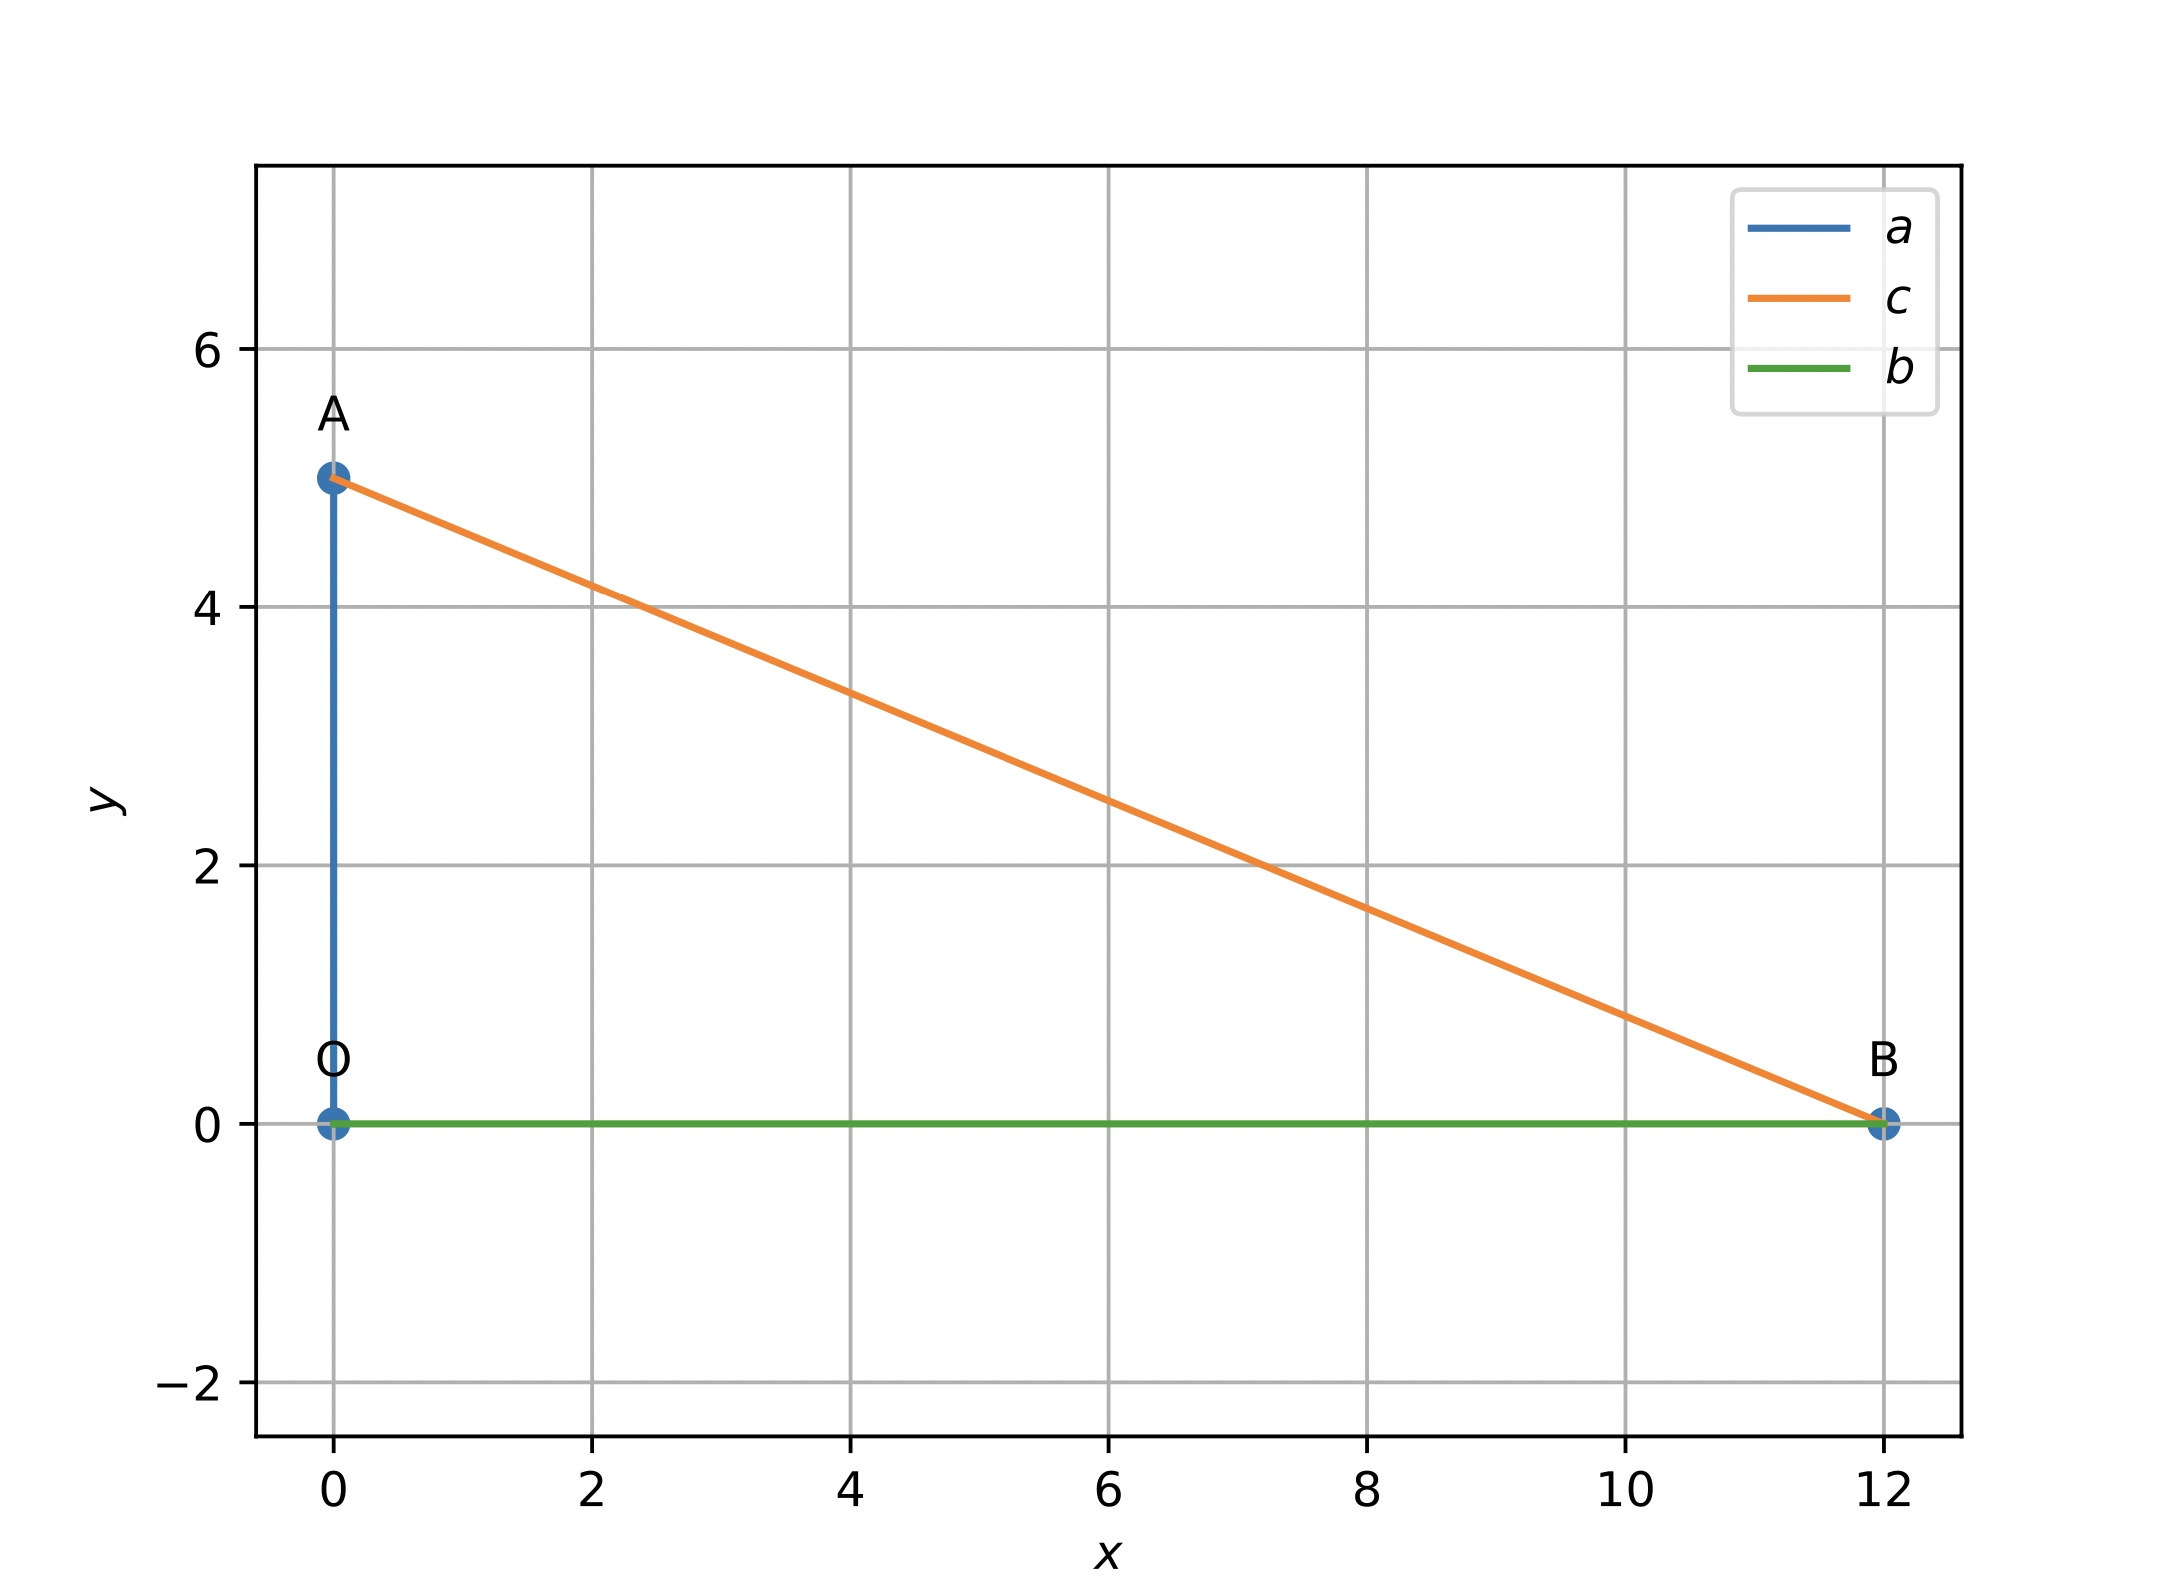
\includegraphics[width=0.5\textwidth]{matrix.jpg}  
 \end{center}\vspace{5mm}
 \vspace{2mm}  
\textbf{implementation}
\begin{center}
\setlength{\arrayrulewidth}{0.5mm}
\setlength{\tabcolsep}{5pt}
\renewcommand{\arraystretch}{3}
    \begin{tabular}{|l|c|}
    \hline 
    \textbf{Equation no} & \textbf{Role} \\ \hline
    5 &  Pythagorean Theorem \\ 
    11 & Matrix form of Linear equation  \\
    16 & Results Identity matrix  \\
    18 & Length of c\\
    19 & Length of a \\
    20 & substituting k=5\\
    \hline
      \end{tabular}
  \end{center} \vspace{2mm}
  
 \vspace{2mm} \textbf{Construction}
\begin{center}
\setlength{\arrayrulewidth}{0.5mm}
\setlength{\tabcolsep}{6pt}
\renewcommand{\arraystretch}{1.5}
    \begin{tabular}{|l|c|}
    \hline 
    \textbf{vertex} & \textbf{coordinates} \\ \hline
   O & $ \begin{pmatrix} 
0 \\
0
\end{pmatrix} $ \\ \hline
    A & $\begin{pmatrix}
0 \\
5
\end{pmatrix}$   \\\hline
    B & $\begin{pmatrix}
12 \\
0
\end{pmatrix} $\\
    \hline
      \end{tabular}
  \end{center}
  
\raggedright  Download the code \\
Github link: \href{https://github.com/chiragshah1244/FWC/blob/main/assignments/assignment-1/code/src/seq.cpp}{Assignment-4}.
  \end{multicols}
\end{document}
\fi

\fi
%
\item Construct a triangle $ABC$ in which $\angle{B}, \angle{C}$ and  $a+b+c=K$ are given.
\label{cons/tri/4}
\\
\solution
\iffalse
\documentclass[10pt,a4paper]{report}
\usepackage[latin1]{inputenc}
\usepackage{amsmath}
\usepackage{amsfonts}
\usepackage{amssymb}
\usepackage{graphicx}
\usepackage{hyperref}
\usepackage{multicol}
\usepackage[margin=0.5in]{geometry}
\usepackage{tikz}
\usepackage[document]{ragged2e}
\usepackage{romannum}
\usetikzlibrary{arrows,shapes.gates.logic.US,shapes.gates.logic.IEC,calc}
\usepackage{titlesec}
\titlespacing{\subsection}{1pt}{\parskip}{3pt}
\titlespacing{\subsubsection}{0pt}{\parskip}{-\parskip}
\titlespacing{\paragraph}{0pt}{\parskip}{\parskip}
\newcommand{\myvec}[1]{\ensuremath{\begin{pmatrix}#1\end{pmatrix}}}



\begin{document}



\begin{multicols}{2}
\raggedright {
\includegraphics[scale=0.06]{IITH logo.jpg}} \vspace{3mm}\\ \raggedleft Name:SHAIK KHAJA MASTAN AHMED\vspace{2mm}\\ \raggedleft Roll No.: FWC22052\vspace{2mm}\\ \raggedleft 19pa1a04e9@vishnu.edu.in \vspace{2mm}\\ \raggedleft Sep 2022 \vspace{5mm}\\

\end{multicols}
\centering \Large \textbf{MATRIX: LINE ASSIGNMENT} \normalsize \vspace{10mm}

\begin{multicols}{2}

\section{Problem:}  
	\begin{figure}[!h]
		\centering
 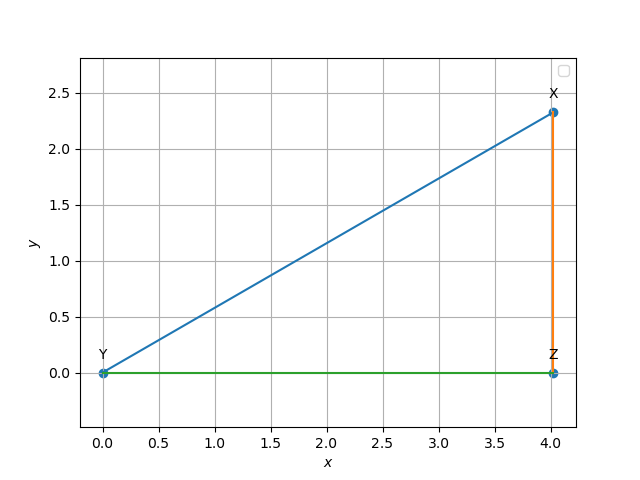
\includegraphics[width=\columnwidth]{chapters/9/11/2/4/figs/line.png}
		\caption{}
		\label{eq:cons/tri/9/11/2/4}
  	\end{figure}
\fi
	From the given information, 
\begin{align}
	a+b+c &= K
	\\
	b\cos C + c \cos B -a &=0
	\\
	b\sin C - c \sin B &=0
\end{align}
resulting in the matrix equation
\begin{align}
	\myvec{
		1 & 1 & 1 
	\\
	\cos C &  \cos B &-1
	\\
	\sin C &-  \sin B & 0
}\myvec{a \\ b \\ c}
= K \vec{e}_1
\end{align}
which can be solved to obtain all the sides.  
\iffalse
	$\triangle ABC$ can then be plotted using
\begin{align}
	\vec{X} = \myvec{a \\ b},
	\vec{Y} = \vec{0},
	\vec{Z} =\myvec{a \\ 0}
\end{align}

\section{Solution: }
\raggedright \textbf{Input Parameters:}\\
\vspace{1mm}
\begin{center}
\begin{tabular}{|c|c|c|}
	\hline
	\textbf{Symbol}&\textbf{Value}&\textbf{Description}\\
	\hline
	XY+YZ+ZX & 11cm & D\\
	\hline 
	$\angle{Z}$ & $90^0$ & Angle at Z \\
	\hline
	$\angle{Y}$ & $30^0$ & Angle at Y \\
	\hline
	
\end{tabular}
\end{center}
\vspace{3mm}



\raggedright Termux Command:\\
               \centering bash rncom.sh (Using Shell)\\
               \vspace{3mm} 

\raggedright \textbf{To Prove:}\\ \vspace{3mm} 
   Given, $\angle{Y}=30^0$, $\angle{Z}=90^0$ and  XY+YZ+ZX = Dcm.\\ \vspace{1mm}
   if $\angle{Y}=30^0$ and $\angle{Z}=90^0$ then $\angle{X}=60^0$\\
   Let us consider the coordinates of Y are X0,Y0 be $\begin{pmatrix}
  0\\
  0 \\
 \end{pmatrix}$% 
 \vspace{1mm} \\ Let 'z' be the distance between X and Y.
 \vspace{1mm} \\ Let the coordinates of X be X1,Y1 respectively.
  \\ \centering i.e., X = z$\begin{pmatrix}
  cos \theta\\
  sin \theta \\
 \end{pmatrix}$% 
 \vspace{2mm}
  \\ \raggedright And the coordinates of Z be X2,Y2 respectively.
  \\ \centering i.e., Z = z$\begin{pmatrix}
  cos \theta\\
  0 \\
 \end{pmatrix}$%
 \vspace{2mm}  \\So, by finding the values of coordinates of the all sides we can form a required triangle. \\
\vspace{2mm}
\raggedright \textbf{Finding the Coordinates: } \\
        \raggedright Given that XY+YZ+ZX=D. \frenchspacing \\
        \raggedright i.e., $||X-Y||$ + $||Y-Z||$ + $||Z-X||$ =D. \\ \vspace{1mm}
 $\implies$ z + zcos$\theta$+ zsin$\theta$ =D\\  
	\begin{center}	
	$\implies$ z = $\frac{D}{1+cos\theta+sin\theta}$
	\end{center}
\centering By solving we get 'z' , [$\because$ $\theta=30^0$ and D=11cm].\\ \vspace{2mm}
 $\therefore$ \text{z = 4.64} .\\ 
\raggedright Calculating the required vertices: \\ \vspace{2mm}
\centering X = z$\begin{pmatrix} 
  cos \theta\\
  sin \theta\\
 \end{pmatrix}$ =4.64 $\begin{pmatrix} 
  cos30^0\\
  sin30^0\\
 \end{pmatrix}$ = $\begin{pmatrix}
                 4.02\\
                 2.32\\
              \end{pmatrix}$ \\ \vspace{2mm}
\centering Z = z$\begin{pmatrix} 
  cos \theta\\
  0\\
 \end{pmatrix}$ = 4.64 $\begin{pmatrix} 
  cos30^0\\
  0\\
 \end{pmatrix}$ = $\begin{pmatrix}
                  4.02\\
                  0\\
              \end{pmatrix}$\\ \vspace{2mm}
\raggedright $\therefore$ The vertices of the required $\Delta$XYZ are:\\ \vspace{2mm}
\centering X= $\begin{pmatrix}
                 4.02\\
                 2.32\\
              \end{pmatrix}$%
              , Y= $\begin{pmatrix}
                 0\\
                 0\\
              \end{pmatrix}$% 
               , Z= $\begin{pmatrix}
                  4.02\\
                  0\\
              \end{pmatrix}$% 
 \vspace{3mm}             
\\
\textbf{The below python code realizes construction:}\\
https://github.com/19pa1a04e9/FWC-IITH/tree/main/Assignment-1/MATRICES/Line/line.py
  
 \section{Plot:}
 	\begin{center}
  \includegraphics[scale=0.55]{line.png}
  	\end{center}
  


  



\vspace{3cm}

\end{multicols}

\end{document}
\fi



\end{enumerate}
